\documentclass[12pt, a4paper]{article}

% Preamble: Load necessary packages
\usepackage{amsmath}
\usepackage{geometry}
\usepackage{graphicx}
\usepackage{tikz}

% Set page margins
\geometry{a4paper, margin=1in}

% Define a command for the section separator
\newcommand{\sectionbreak}{\clearpage}

\title{New Magnetic Field Problems and Solutions}
\author{}
\date{}

\begin{document}

\maketitle

\section{Problem 1: Magnetic Field from Moving Charges}

\subsection*{(a) Orbiting Alpha Particle}
\textbf{Question:} An alpha particle ($q = +2e$, $m = 6.64 \times 10^{-27}$ kg) is in a stable circular orbit of radius $1.0 \times 10^{-12}$ m around a fixed heavy nucleus. Its orbital speed is $3.0 \times 10^6$ m/s. What is the magnitude of the magnetic field produced at the center of the orbit (at the nucleus)?

\subsubsection*{Explanation}
The orbiting alpha particle constitutes a circular current. We can find this equivalent current by calculating how much charge passes a point in the orbit per unit time. Once we have the current, we can use the formula for the magnetic field at the center of a current loop, $B = \frac{\mu_0 I}{2r}$.

\subsubsection*{Solution}
\begin{enumerate}
    \item \textbf{Find the period of revolution ($T$):}
    \begin{equation*}
        T = \frac{2\pi r}{v} = \frac{2\pi (1.0 \times 10^{-12} \text{ m})}{3.0 \times 10^6 \text{ m/s}} \approx 2.094 \times 10^{-18} \text{ s}
    \end{equation*}
    \item \textbf{Find the equivalent current ($I$):}
    \begin{equation*}
        I = \frac{q}{T} = \frac{2 \times (1.60 \times 10^{-19} \text{ C})}{2.094 \times 10^{-18} \text{ s}} \approx 0.153 \text{ A}
    \end{equation*}
    \item \textbf{Calculate the magnetic field ($B$):}
    \begin{equation*}
        B = \frac{\mu_0 I}{2r} = \frac{(4\pi \times 10^{-7} \text{ T·m/A})(0.153 \text{ A})}{2(1.0 \times 10^{-12} \text{ m})} \approx 9.61 \times 10^4 \text{ T}
    \end{equation*}
\end{enumerate}

\subsection*{(b) Spinning Charged Cylinder}
\textbf{Question:} A solid insulating cylinder of radius $R$ and length $L$ has a uniform volume charge density $\rho$. It rotates about its central axis with an angular velocity $\omega$. Derive an expression for the magnetic field at the center of one of its circular faces.

\subsubsection*{Explanation}
We model the cylinder as a stack of infinitesimally thin, spinning circular discs. We integrate the known on-axis field from each disc along the length of the cylinder to find the total magnetic field.

\subsubsection*{Solution}
\begin{enumerate}
    \item The magnetic field on the axis from a spinning disc of radius $R$, thickness $dz$, and volume charge density $\rho$, at a distance $z$, is given by:
    \begin{equation*}
        dB = \frac{\mu_0 (\rho dz) \omega R^2}{4\sqrt{R^2+z^2}}
    \end{equation*}
    \item To find the total field at the center of one face, we integrate from $z=0$ to $z=L$:
    \begin{align*}
        B &= \int_0^L \frac{\mu_0 \rho \omega R^2}{4\sqrt{R^2+z^2}} dz \\
        &= \frac{\mu_0 \rho \omega R^2}{4} \left[ \ln\left(z + \sqrt{R^2+z^2}\right) \right]_0^L \\
        &= \frac{\mu_0 \rho \omega R^2}{4} \ln\left(\frac{L+\sqrt{R^2+L^2}}{R}\right)
    \end{align*}
\end{enumerate}

\sectionbreak

\section{Problem 2: Deflection of an Electron Beam}

\textbf{Question:} An electron beam is accelerated from rest through a potential difference of 500 V. It then enters a region of uniform magnetic field of strength $B=0.01$ T. The field is directed into the page, and the region has a width of $d=5.0$ cm. The electrons enter the field perpendicular to its boundary. Calculate the vertical displacement, $y$, of the beam as it emerges from the field.

\begin{center}
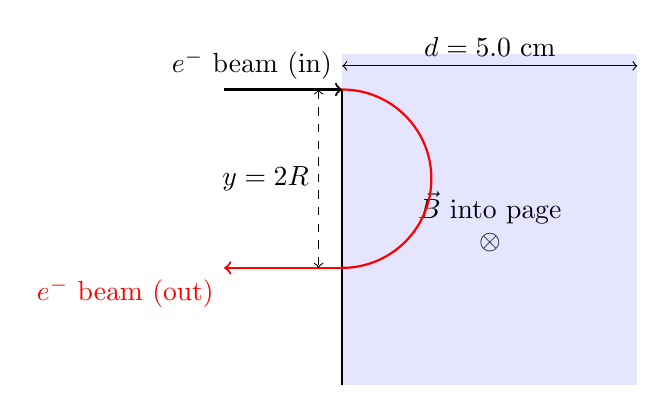
\begin{tikzpicture}[scale=1.5]
    % Define dimensions based on the problem
    \def\fieldwidth{2.5} % Represents 5.0 cm, scale is 2cm/unit
    \def\radius{0.755}   % Represents R=0.755 cm, but scaled for visibility
    \def\ydisp{\radius*2} % Represents y=2R

    % Draw the magnetic field region
    \fill[blue!10] (0,0.3) rectangle (\fieldwidth, -2.5);
    \draw[<->] (0, 0.2) -- (\fieldwidth, 0.2) node[midway, above] {$d = 5.0$ cm};
    \draw[thick] (0,0) -- (0, -2.5); % Left edge of field
    \node at (1.25, -1) {$\vec{B}$ into page};
    \node at (1.25, -1.3) {$\otimes$};

    % Draw incoming electron beam
    \draw[->, thick] (-1,0) -- (0,0) node[above left] {$e^-$ beam (in)};

    % Draw the semi-circular path
    % The electron enters at (0,0), force is down, so it curves down and left.
    % Center of circle is at (0, -R). Path is a clockwise semi-circle.
    % The arc command starts at (0,0) and draws an arc from 90 deg to -90 deg with radius R.
    \draw[thick, red] (0,0) arc (90:-90:\radius);

    % Draw outgoing beam
    \draw[->, thick, red] (0, -\ydisp) -- (-1, -\ydisp) node[below left] {$e^-$ beam (out)};

    % Add labels for displacement
    \draw[<->, dashed] (-0.2, 0) -- (-0.2, -\ydisp) node[midway, left] {$y = 2R$};
\end{tikzpicture}
\end{center}

\subsubsection*{Explanation}
First, we find the electron's speed by equating kinetic energy gained to electrical potential energy lost ($KE=eV$). Then, inside the magnetic field, the electrons follow a circular path with radius $R = \frac{m_ev}{eB}$. Since the calculated radius ($R=0.755$ cm) is smaller than the width of the field ($d=5.0$ cm), the electron completes a semi-circle and exits on the same side it entered. The vertical displacement will therefore be equal to the diameter of the circular path ($2R$).

\subsubsection*{Solution}
\begin{enumerate}
    \item \textbf{Find the electron's speed ($v$):}
    \begin{equation*}
        v = \sqrt{\frac{2eV}{m_e}} = \sqrt{\frac{2(1.60 \times 10^{-19})(500)}{9.11 \times 10^{-31}}} \approx 1.326 \times 10^7 \text{ m/s}
    \end{equation*}
    \item \textbf{Calculate the radius of the circular path ($R$):}
    \begin{equation*}
        R = \frac{m_e v}{eB} = \frac{(9.11 \times 10^{-31})(1.326 \times 10^7)}{(1.60 \times 10^{-19})(0.01)} \approx 0.00755 \text{ m} = 0.755 \text{ cm}
    \end{equation*}
    \item \textbf{Determine the vertical displacement ($y$):}
    \begin{equation*}
        y = 2R = 2 \times 0.755 \text{ cm} = 1.51 \text{ cm}
    \end{equation*}
\end{enumerate}

\sectionbreak

\section{Problem 3: Designing a Velocity Filter}

\textbf{Question:} A mass spectrometer needs to sort singly ionized lithium atoms ($^{6}$Li and $^{7}$Li). It is designed to allow ions with a speed of $4.0 \times 10^5$ m/s to pass undeflected through its velocity filter. The magnetic field in the filter is a uniform 0.8 T.
(a) What must be the magnitude of the electric field in the filter?
(b) If the plates that create the electric field are separated by 2.0 cm, what potential difference must be applied across them?

\begin{center}
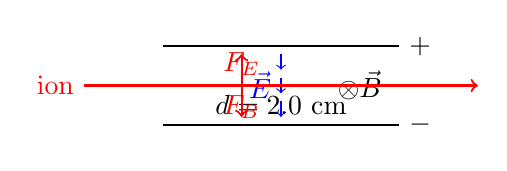
\begin{tikzpicture}
    % Plates
    \draw[thick] (0,1) -- (3,1) node[right]{$+$};
    \draw[thick] (0,0) -- (3,0) node[right]{$-$};
    \node at (1.5, 0.5) [below] {$d=2.0$ cm};
    % E-field
    \foreach \y in {0.2, 0.5, 0.8}
        \draw[->, blue] (1.5, \y+0.1) -- (1.5, \y-0.1);
    \node[blue, left] at (1.5, 0.5) {$\vec{E}$};
    % B-field
    \node at (2.5, 0.5) {$\otimes \vec{B}$};
    % Ion path
    \draw[->, thick, red] (-1, 0.5) node[left]{ion} -- (4, 0.5);
    \node[above, red] at (1, 0.5) {$F_E$};
    \node[below, red] at (1, 0.5) {$F_B$};
    \draw[->, thick, red] (1, 0.5) -- (1, 0.9);
    \draw[->, thick, red] (1, 0.5) -- (1, 0.1);
\end{tikzpicture}
\end{center}

\subsubsection*{Explanation}
In a velocity filter, the magnetic force ($F_B = qvB$) and the electric force ($F_E = qE$) are equal and opposite for the selected velocity. This condition allows us to find the required electric field. The potential difference is then found using the relationship $E = V/d$.

\subsubsection*{Solution}
\begin{enumerate}
    \item[(a)] \textbf{Find the electric field ($E$):}
    \begin{align*}
        E = vB &= (4.0 \times 10^5 \text{ m/s})(0.8 \text{ T}) = 3.2 \times 10^5 \text{ V/m}
    \end{align*}
    \item[(b)] \textbf{Find the potential difference ($V$):}
    \begin{align*}
        V = E \cdot d &= (3.2 \times 10^5 \text{ V/m})(0.02 \text{ m}) = 6400 \text{ V}
    \end{align*}
\end{enumerate}

\sectionbreak

\section{Problem 4: Oscillating Current Loop}

\textbf{Question:} A circular coil with 50 turns, a radius of 10 cm, and carrying a current of 2.0 A is placed in a uniform magnetic field of 0.25 T. The coil is pivoted about an axis that lies in the plane of the coil and passes through its center. A torsional spring with spring constant $\kappa = 0.50$ N·m/rad is attached to the pivot. In the equilibrium position, the plane of the coil is perpendicular to the magnetic field. The coil is rotated by 60 degrees from its equilibrium position and released from rest.
(a) What is the magnitude of the initial magnetic torque on the loop?
(b) What is the effective torsional constant for small oscillations around the equilibrium point?

\subsubsection*{Explanation}
When the coil is displaced, both the B-field and the spring exert a restoring torque. The total restoring torque is $\tau_{net} = \tau_B + \tau_s$. For small angles, we can approximate $\sin\theta \approx \theta$, and the net torque becomes proportional to $-\theta$, defining an effective torsional constant.

\subsubsection*{Solution}
\begin{enumerate}
    \item[(a)] \textbf{Calculate initial magnetic torque ($\tau_{B, initial}$):}
    \begin{itemize}
        \item Magnetic dipole moment $\mu = NIA = 50(2.0)\pi(0.10)^2 = 3.14 \text{ A·m}^2$.
        \item Initial angle $\theta = 60^\circ$.
        \begin{equation*}
            \tau_{B, initial} = \mu B \sin\theta = (3.14)(0.25)\sin(60^\circ) \approx 0.68 \text{ N·m}
        \end{equation*}
    \end{itemize}
    \item[(b)] \textbf{Find the effective torsional constant ($k_{eff}$):}
    \begin{itemize}
        \item The net restoring torque is $\tau_{net} = -(\mu B \sin\theta + \kappa\theta)$.
        \item For small angles $\theta$ in radians, $\sin\theta \approx \theta$.
        \begin{equation*}
            \tau_{net} \approx -(\mu B + \kappa)\theta
        \end{equation*}
        \item The effective torsional constant is the coefficient of the $-\theta$ term.
        \begin{align*}
            k_{eff} &= \mu B + \kappa = (3.14)(0.25) + 0.50 = 1.285 \text{ N·m/rad}
        \end{align*}
    \end{itemize}
\end{enumerate}

\sectionbreak

\section{Problem 5: Thermionic Emission and Magnetic Fields}

\textbf{Question:} Electrons are emitted from a hot filament with negligible initial speed and are accelerated through a potential difference of 2.0 kV. They then enter a uniform magnetic field of $4.0 \times 10^{-3}$ T, moving perpendicular to the field lines.
(a) What is the speed of the electrons as they enter the magnetic field?
(b) What is the radius of the circular path they follow inside the field?

\subsubsection*{Explanation}
First, use conservation of energy ($KE = eV$) to find the velocity of the electrons after acceleration. Then, use the formula for the radius of a charged particle's circular path in a magnetic field, $R = \frac{mv}{qB}$, derived by equating the magnetic force to the centripetal force.

\subsubsection*{Solution}
\begin{enumerate}
    \item[(a)] \textbf{Find the speed of the electrons ($v$):}
    \begin{align*}
        v = \sqrt{\frac{2eV}{m_e}} = \sqrt{\frac{2(1.60 \times 10^{-19} \text{ C})(2000 \text{ V})}{9.11 \times 10^{-31} \text{ kg}}} \approx 2.65 \times 10^7 \text{ m/s}
    \end{align*}
    \item[(b)] \textbf{Find the radius of the path ($R$):}
    \begin{align*}
        R = \frac{m_e v}{eB} = \frac{(9.11 \times 10^{-31} \text{ kg})(2.65 \times 10^7 \text{ m/s})}{(1.60 \times 10^{-19} \text{ C})(4.0 \times 10^{-3} \text{ T})} \approx 0.0377 \text{ m} \text{ or } 3.77 \text{ cm}
    \end{align*}
\end{enumerate}

\end{document}